\documentclass{article}

\usepackage[american]{babel}
\usepackage[autostyle]{csquotes}

\usepackage[colorlinks=true, allcolors=blue]{hyperref}
\usepackage{indentfirst}

\usepackage{amsmath}
\usepackage{graphicx}

\usepackage[backend=biber, dateabbrev=false]{biblatex}
\addbibresource{papers.bib}



\title{TPM 2.0 Key Certification}
\author{Sarah Lavinia Johnson}

\begin{document}
\maketitle

\section*{Relevant Background Definitions}
\subsection*{Key Attributes}
FixedTPM: non-duplicable 

Restricted: operations are limited to TPM-generated data

\subsection*{Key Types}
Primary: Created by TPM based on the current Primary Seed when executing the TPM2\_CreatePrimary command. May be persisted within the TPM. Otherwise must be recreated after a TPM reset.

Ordinary: Created by TPM based on seed taken from the RNG when executing the TPM2\_Create command. Must be the child of another key. May be persisted within the TPM or persisted external to the TPM in the form of an encrypted key blob. The blob is only loadable using the parent key's authorization.

\subsection*{Certificates}
X.509 Digital Certificate

Public key and data about the subject (i.e., identity) signed by a certificate authority

Validating a certificate requires a certificate chain in order to verify a chain of trust to a trust anchor (e.g., a root certificate)







\section*{Secure Device Identifiers}
\subsection*{Definition}
Identifier that is cryptographically bound to a device

\subsection*{Requirements}
Attestation Key (AK): FixedTPM Restricted signing key

Device Identification Key (DevID): FixedTPM non-Restricted signing key

\subsection*{Initial Keys (IAK/IDevID)}
Created by OEM at manufacturing time

Should be Primary keys

Recommended to be used only for enrollment of an LAK/LDevID

Typically the IAK certificate is the trust anchor for certificates created later

\subsection*{Local Keys (LAK/LDevID)}
Created by owner

Should be Ordinary keys

Recommended to be used only for one application

\subsection*{Note regarding Endorsement Key (EK)}
Cannot be used as a secure device identifier because it is a storage key (not a signing key) and identifies a TPM (not a device)

\section*{Relationships of Keys/Certificates}
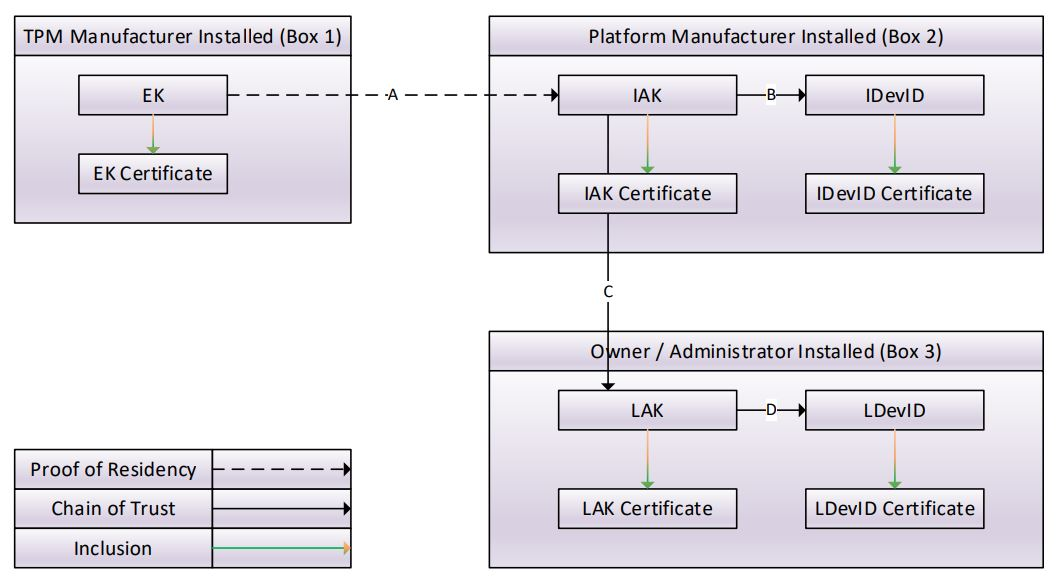
\includegraphics[scale=0.6]{certificateRelationships.jpg}

Box 1: The EK Certificate is signed by the TPM Manufacturer's CA and binds the EK to a specific TPM

Line A: The IAK is verified by the OEM's CA to have the correct key properties and to be resident in the same TPM as the EK

Line B: The IDevID is verified by the OEM's CA to have the correct key properties and to be resident in the same TPM as the IAK

Box 2: The IAK Certificate and IDevID Certificate is signed by the OEM's CA and binds the IAK and IDevID to a specific device

Line C: The LAK is verified by the Owner's CA to have the correct key properties and to be resident in the same TPM as the IAK

Line D: The LDevID is verified by the Owner's CA to have the correct key properties and to be resident in the same TPM as the LAK

Box 3: The LAK Certificate and LDevID Certificate is signed by the Owner's CA

\iffalse
\subsection*{extra}

Prove a new key belongs to a specific device: 1) binding the TPM to the OEM device and 2) binding an AK to a TPM using the EK

An AK certificate is the trust anchor for certificates created later (because it is the certificate that ties a new key to the same TPM containing both keys)

The OEM CA makes an assertion by signing an IAK certificate that is a primary security dependency for later DevID certificate creation

An OEM-supplied IAK certificate is a definitive assertion to applications that need proof that the IAK belongs to a specific device
\fi




\section*{Certificate Authority}
\subsection*{General Requirements}
Must verify TPM residency of a key

Should support a standard certificate tranport protocol that provides protection from replay attacks and provides confidentiality and integrity (e.g., Enrollment over Secure Transport (EST))


\subsection*{OEM Creation of IAK Certificate based on EK Certificate}

Procedure assures that the new IAK is resident in the same TPM as the EK and that the EK resident in this TPM corresponds to the EK certificate
\bigskip

\textbf{Detailed Procedure}
\begin{enumerate}
    \setcounter{enumi}{-1}
    \item The OEM creates and loads the IAK (a FixedTPM Restricted Signing key)
    \item The OEM builds the certificate signing request (i.e., the TCG-CSR-IDEVID structure) containing
    \begin{enumerate}
        \item Platform identity information (includes the device model and serial number)
        \item The EK certificate
        \item The IAK public area
    \end{enumerate}
    \item The OEM uses TPM2\_Hash on the CSR so that the IAK can sign it (since IAK is Restricted)
    \item The OEM uses TPM2\_Sign on the hash of the CSR using the IAK (proves control of the IAK to the CA)
    \item The OEM sends the CSR and the signed hash of the CSR to the CA
    \item The CA verifies the received data by
    \begin{enumerate}
        \item Checking that the hash matches the CSR
        \item Checking the signature on the hash of the CSR using the IAK public key (extracted from the CSR)
        \item Checking the signature on the the EK certificate using the TPM manufacturer's CA public key
        \item Verifying the attributes of the IAK
    \end{enumerate}
    \item The CA uses TPM2\_Hash on the IAK public area to calculate the cryptographic name of the IAK
    \item The CA uses TPM2\_GetRandom to generate a nonce
    \item The CA uses TPM2\_MakeCredential to produce an encrypted credential blob containing
    \begin{enumerate}
        \item The cryptographic name of the IAK
        \item Secret nonce
        \item Encrypted with the EK
    \end{enumerate}
    \item The CA sends the encrypted credential blob to the OEM
    \item The OEM uses TPM2\_ActivateCredential command to release the nonce by
    \begin{enumerate}
        \item Decrypting the credential blob using the EK (proves the EK is loaded on the TPM)
        \item Verifying the name of the IAK (proves the IAK private part is loaded on the same TPM)
    \end{enumerate}
    \item The OEM returns the nonce to the CA
    \item The CA verifies the nonces match
    \item The CA issues the IAK certificate
\end{enumerate}
\bigskip

\textbf{Symbolic Representation}
\begin{enumerate}
    \setcounter{enumi}{-1}
    \item OEM executes TPM2\_CreatePrimary to get IAK, $\text{IAK}^{-1}$
    \item OEM makes TCG\_CSR\_IDevID containing
    \begin{enumerate}
        \item deviceInfo = (prodModel, prodSerial)
        \item $\text{cert}_{\text{EK}} = [(\text{EK}, \text{tpmInfo})]_{\text{TM\_CA}^{-1}}$
        \item IAK
    \end{enumerate}
    \item OEM executes TPM2\_Hash to get $\text{\#CSR}$
    \item OEM executes TPM2\_Sign to get $[\text{\#CSR}]_{\text{IAK}^{-1}}$
    \item OEM sends CSR and $[\text{\#CSR}]_{\text{IAK}^{-1}}$ to CA
    \item CA verifies CSR and $[\text{\#CSR}]_{\text{IAK}^{-1}}$
    \begin{enumerate}
        \item ChechHash \#CSR with CSR
        \item CheckSig $[\text{\#CSR}]_{\text{IAK}^{-1}}$ with IAK
        \begin{enumerate}
          \item Extract IAK from CSR
        \end{enumerate}
        \item CheckSig $\text{cert}_\text{EK}$ with TPM\_CA
        \item check attributes of IAK
    \end{enumerate}
    \item CA executes TPM2\_Hash to get \#IAK
    \item CA executes TPM2\_GetRandom to get r
    \item CA executes TPM2\_MakeCredential to get $\{\text{cred}_\text{IAK}\}_\text{EK}$ with $\text{cred}_\text{IAK}$ containing
    \begin{enumerate}
        \item \#IAK
        \item r
    \end{enumerate}
    \item CA sends $\{\text{cred}_\text{IAK}\}_\text{EK}$ to OEM
    \item OEM executes TPM2\_ActivateCredential to get r'
    \begin{enumerate}
        \item Decrypt $\{\text{cred}_\text{IAK}\}_\text{EK}$ with $\text{EK}^{-1}$
        \item Check \#IAK
    \end{enumerate}
    \item OEM sends r' to CA
    \item CA checks r' = r
    \item CA sends $\text{cert}_{\text{IAK}} = [(\text{IAK}, \text{deviceInfo})]_{\text{OEM\_CA}^{-1}}$ to OEM
\end{enumerate}

\subsection*{Owner Creation of LAK Certificate based on IAK Certificate}

Procedure assures that the new LAK is resident in the same TPM as the IAK
\bigskip

\textbf{Detailed Procedure}
\begin{enumerate}
    \setcounter{enumi}{-1}
    \item The Owner creates and loads the LAK (a FixedTPM Restricted Signing key)
    \item The Owner uses TPM2\_Certify to produce a signed TPM2B\_Attest structure (proves the LAK is loaded on the same TPM as the IAK)
    \item The Owner builds the certificate signing request (i.e., the TCG-CSR-LDEVID structure) containing
    \begin{enumerate}
        \item The signed TPM2B\_Attest structure
        \item The IAK certificate
    \end{enumerate}
    \item The Owner uses TPM2\_Hash on the CSR so that the LAK can sign it (since LAK is Restricted)
    \item The Owner uses TPM2\_Sign on the hash of the CSR using the LAK (proves control of the LAK to the CA)
    \item Owner sends the CSR and the signed hash of the CSR to the CA
    \item The CA verifies the received data by
    \begin{enumerate}
        \item Checking that the hash matches the CSR
        \item Checking the signature on the hash of the CSR using the LAK public key (extracted from the TPM2B\_Attest structure)
        \item Checking the signature on the TPM2B\_Attest structure using the IAK public key (extracted from the IAK certificate)
        \item Checking the signature on the IAK certificate using the OEM's CA public key
        \item Verify the attributes of the LAK
    \end{enumerate}
    \item The CA issues the LAK certificate
\end{enumerate}
\bigskip

\textbf{Symbolic Representation}
\begin{enumerate}
    \setcounter{enumi}{-1}
    \item Owner executes TPM2\_Create to get LAK, $\text{LAK}^{-1}$
    \item Owner executes TPM2\_Certify to get $[\text{TPM2B\_Attest}_\text{LAK}]_{\text{IAK}^{-1}}$
    \item Owner makes TCG\_CSR\_LDevID containing
    \begin{enumerate}
        \item $[\text{TPM2B\_Attest}_\text{LAK}]_{\text{IAK}^{-1}}$
        \item $\text{cert}_\text{IAK} = [(\text{IAK}, \text{deviceInfo})]_{\text{OEM\_CA}^{-1}}$
    \end{enumerate}
    \item Owner executes TPM2\_Hash to get $\text{\#CSR}$
    \item Owner executes TPM2\_Sign to get $[\text{\#CSR}]_{\text{LAK}^{-1}}$
    \item Owner sends CSR and $[\text{\#CSR}]_{\text{LAK}^{-1}}$ to CA
    \item CA verifies CSR and $[\text{\#CSR}]_{\text{LAK}^{-1}}$
    \begin{enumerate}
        \item CheckHash \#CSR with CSR
        \item CheckSig $[\text{\#CSR}]_{\text{LAK}^{-1}}$ with LAK
        \begin{enumerate}
          \item Extract LAK from $[\text{TPM2B\_Attest}_\text{LAK}]_{\text{IAK}^{-1}}$ in CSR
        \end{enumerate}
        \item CheckSig $[\text{TPM2B\_Attest}_\text{LAK}]_{\text{IAK}^{-1}}$ with IAK
        \begin{enumerate}
          \item Extract IAK from $\text{cert}_\text{IAK}$ in CSR
        \end{enumerate}
        \item CheckSig $\text{cert}_\text{IAK}$ with OEM\_CA
        \item check attributes of LAK
    \end{enumerate}
    \item The CA sends $\text{cert}_{\text{LAK}} = [(\text{LAK}, \text{deviceInfo})]_{\text{Owner\_CA}^{-1}}$ to Owner
\end{enumerate}

\section*{Related Works}
TPM 2.0 Keys for Device Identity and Attestation \cite{certSpec}

Trusted Platform Module Library Specification, Family 2.0 \cite{tpmSpec}

Formal Analysis of Protocols Based on TPM State Registers \cite{pcrModel}

Automated Proof for Authorization Protocols of TPM 2.0 in Computational Model \cite{authModel}


\printbibliography



\end{document}